%% abtex2-modelo-trabalho-academico.tex, v-1.9.2 laurocesar
%% Copyright 2012-2014 by abnTeX2 group at http://abntex2.googlecode.com/ 
%%
%% This work may be distributed and/or modified under the
%% conditions of the LaTeX Project Public License, either version 1.3
%% of this license or (at your option) any later version.
%% The latest version of this license is in
%%   http://www.latex-project.org/lppl.txt
%% and version 1.3 or later is part of all distributions of LaTeX
%% version 2005/12/01 or later.
%%
%% This work has the LPPL maintenance status `maintained'.
%% 
%% The Current Maintainer of this work is the abnTeX2 team, led
%% by Lauro César Araujo. Further information are available on 
%% http://abntex2.googlecode.com/
%%
%% This work consists of the files abntex2-modelo-trabalho-academico.tex,
%% abntex2-modelo-include-comandos and abntex2-modelo-references.bib
%%

% ------------------------------------------------------------------------
% ------------------------------------------------------------------------
% abnTeX2: Modelo de Trabalho Academico (tese de doutorado, dissertacao de
% mestrado e trabalhos monograficos em geral) em conformidade com 
% ABNT NBR 14724:2011: Informacao e documentacao - Trabalhos academicos -
% Apresentacao
% ------------------------------------------------------------------------
% ------------------------------------------------------------------------

\documentclass[
	% -- opções da classe memoir --
	12pt,				% tamanho da fonte
	openright,			% capítulos começam em pág ímpar (insere página vazia caso preciso)
	twoside,			% para impressão em verso e anverso. Oposto a oneside
	a4paper,			% tamanho do papel. 
	% -- opções da classe abntex2 --
	%chapter=TITLE,		% títulos de capítulos convertidos em letras maiúsculas
	%section=TITLE,		% títulos de seções convertidos em letras maiúsculas
	%subsection=TITLE,	% títulos de subseções convertidos em letras maiúsculas
	%subsubsection=TITLE,% títulos de subsubseções convertidos em letras maiúsculas
	% -- opções do pacote babel --
	english,			% idioma adicional para hifenização
	french,				% idioma adicional para hifenização
	spanish,			% idioma adicional para hifenização
	brazil				% o último idioma é o principal do documento
	]{abntex2}

% ---
% Pacotes básicos 
% ---
\usepackage{lmodern}			% Usa a fonte Latin Modern			
\usepackage[T1]{fontenc}		% Selecao de codigos de fonte.
\usepackage[utf8]{inputenc}		% Codificacao do documento (conversão automática dos acentos)
\usepackage{lastpage}			% Usado pela Ficha catalográfica
\usepackage{indentfirst}		% Indenta o primeiro parágrafo de cada seção.
\usepackage{color}				% Controle das cores
\usepackage{graphicx}			% Inclusão de gráficos
\usepackage{microtype} 			% para melhorias de justificação        
\usepackage{amsmath, amsthm}
\usepackage{amsfonts}
\usepackage{caption}
\usepackage{esvect}
\usepackage{float}
\usepackage{blkarray}
% ---
		
% ---
% Pacotes adicionais, usados apenas no âmbito do Modelo Canônico do abnteX2
% ---
\usepackage{lipsum}				% para geração de dummy text
% ---

% ---
% Pacotes de citações
% ---
\usepackage[brazilian,hyperpageref]{backref}	 % Paginas com as citações na bibl
\usepackage[alf]{abntex2cite}	% Citações padrão ABNT

% --- 
% CONFIGURAÇÕES DE PACOTES
% --- 

% ---
% Configurações do pacote backref
% Usado sem a opção hyperpageref de backref
\newtheorem{teorema}{Teorema}[section]
\newtheorem{exemplo}{Exemplo}[section]
\newtheorem{definicao}{Definição}[section]
\newtheorem{proposicao}{Proposição}[section]
\newtheorem{corolario}{Corolário}[section]
\newtheorem{lema}{Lema}[section]
\newtheorem{observacao}{Observação}[section]
\newcommand {\dem}{\textbf{Demonstração:} }
\newcommand {\afi}{\textbf{Afirmação:} }
\renewcommand{\backrefpagesname}{Citado na(s) página(s):~}
\newcommand\scalemath[2]{\scalebox{#1}{\mbox{\ensuremath{\displaystyle #2}}}}
% Texto padrão antes do número das páginas
\renewcommand{\backref}{}
% Define os textos da citação
\renewcommand*{\backrefalt}[4]{
	\ifcase #1 %
		Nenhuma citação no texto.%
	\or
		Citado na página #2.%
	\else
		Citado #1 vezes nas páginas #2.%
	\fi}%
% ---

% ---
% Informações de dados para CAPA e FOLHA DE ROSTO
% ---
\titulo{Relatório Final de Iniciação Científica}
\autor{Ricardo Emanuel Mueller}
\local{Blumenau}
\data{15 de Novembro de 2018}
\instituicao{%
  Universidade Federal de Santa Catarina
  \par
  Curso de Licenciatura em Matemática
  \par
  Programa de Graduação}

\tipotrabalho{Relatório de Estágio}
% O preambulo deve conter o tipo do trabalho, o objetivo, 
% o nome da instituição e a área de concentração 
\preambulo{Trabalho final de iniciação científica sob orientação do Prof. Dr. Felipe Delfini Caetano Fidalgo.}
% ---


% ---
% Configurações de aparência do PDF final

% alterando o aspecto da cor azul
\definecolor{blue}{RGB}{41,5,195}

% informações do PDF
\makeatletter
\hypersetup{
     	%pagebackref=true,
		pdftitle={\@title}, 
		pdfauthor={\@author},
    	pdfsubject={\imprimirpreambulo},
	    pdfcreator={LaTeX with abnTeX2},
		pdfkeywords={abnt}{latex}{abntex}{abntex2}{trabalho acadêmico}, 
		colorlinks=true,       		% false: boxed links; true: colored links
    	linkcolor=blue,          	% color of internal links
    	citecolor=blue,        		% color of links to bibliography
    	filecolor=magenta,      		% color of file links
		urlcolor=blue,
		bookmarksdepth=4
}
\makeatother
% --- 

% --- 
% Espaçamentos entre linhas e parágrafos 
% --- 

% O tamanho do parágrafo é dado por:
\setlength{\parindent}{1.3cm}

% Controle do espaçamento entre um parágrafo e outro:
\setlength{\parskip}{0.2cm}  % tente também \onelineskip

% ---
% compila o indice
% ---
\makeindex
% ---

% ----
% Início do documento
% ----
\begin{document}

% Retira espaço extra obsoleto entre as frases.
\frenchspacing 

% ----------------------------------------------------------
% ELEMENTOS PRÉ-TEXTUAIS
% ----------------------------------------------------------
% \pretextual

% ---
% Capa
% ---
\imprimircapa
% ---

% ---
% Folha de rosto
% (o * indica que haverá a ficha bibliográfica)
% ---
\imprimirfolhaderosto*
% ---

% ---
% Inserir a ficha bibliografica
% ---

% Isto é um exemplo de Ficha Catalográfica, ou ``Dados internacionais de
% catalogação-na-publicação''. Você pode utilizar este modelo como referência. 
% Porém, provavelmente a biblioteca da sua universidade lhe fornecerá um PDF
% com a ficha catalográfica definitiva após a defesa do trabalho. Quando estiver
% com o documento, salve-o como PDF no diretório do seu projeto e substitua todo
% o conteúdo de implementação deste arquivo pelo comando abaixo:
%
% \begin{fichacatalografica}
%     \includepdf{fig_ficha_catalografica.pdf}
% \end{fichacatalografica}
%\begin{fichacatalografica}
%	\vspace*{\fill}					% Posição vertical
%	\hrule							% Linha horizontal
%	\begin{center}					% Minipage Centralizado
%	\begin{minipage}[c]{12.5cm}		% Largura
%	
%	\imprimirautor
%	
%	\hspace{0.5cm} \imprimirtitulo  / \imprimirautor. --
%	\imprimirlocal, \imprimirdata-
%	
%	\hspace{0.5cm} \pageref{LastPage} p. : il. (algumas color.) ; 30 cm.\\
%	
%	\hspace{0.5cm} \imprimirorientadorRotulo~\imprimirorientador\\
%	
%	\hspace{0.5cm}
%	\parbox[t]{\textwidth}{\imprimirtipotrabalho~--~\imprimirinstituicao,
%	\imprimirdata.}\\
%	
%	\hspace{0.5cm}
%		1. Palavra-chave1.
%		2. Palavra-chave2.
%		I. Orientador.
%		II. Universidade xxx.
%		III. Faculdade de xxx.
%		IV. Título\\ 			
%	
%	\hspace{8.75cm} CDU 02:141:005.7\\
%	
%	\end{minipage}
%	\end{center}
%	\hrule
%\end{fichacatalografica}
% ---

% ---
% Inserir errata
% ---
% \begin{errata}
% Elemento opcional da \citeonline[4.2.1.2]{NBR14724:2011}. Exemplo:

% \vspace{\onelineskip}

% FERRIGNO, C. R. A. \textbf{Tratamento de neoplasias ósseas apendiculares com
% reimplantação de enxerto ósseo autólogo autoclavado associado ao plasma
% rico em plaquetas}: estudo crítico na cirurgia de preservação de membro em
% cães. 2011. 128 f. Tese (Livre-Docência) - Faculdade de Medicina Veterinária e
% Zootecnia, Universidade de São Paulo, São Paulo, 2011.

% \begin{table}[htb]
% \center
% \footnotesize
% \begin{tabular}{|p{1.4cm}|p{1cm}|p{3cm}|p{3cm}|}
%   \hline
%    \textbf{Folha} & \textbf{Linha}  & \textbf{Onde se lê}  & \textbf{Leia-se}  \\
%     \hline
%     1 & 10 & auto-conclavo & autoconclavo\\
%    \hline
% \end{tabular}
% \end{table}

% \end{errata}
% ---

% ---
% Inserir folha de aprovação
% ---

% Isto é um exemplo de Folha de aprovação, elemento obrigatório da NBR
% 14724/2011 (seção 4.2.1.3). Você pode utilizar este modelo até a aprovação
% do trabalho. Após isso, substitua todo o conteúdo deste arquivo por uma
% imagem da página assinada pela banca com o comando abaixo:
%
% \includepdf{folhadeaprovacao_final.pdf}
%
% \begin{folhadeaprovacao}

%   \begin{center}
%     {\ABNTEXchapterfont\large\imprimirautor}

%     \vspace*{\fill}\vspace*{\fill}
%     \begin{center}
%       \ABNTEXchapterfont\bfseries\Large\imprimirtitulo
%     \end{center}
%     \vspace*{\fill}
    
%     \hspace{.45\textwidth}
%     \begin{minipage}{.5\textwidth}
%         \imprimirpreambulo
%     \end{minipage}%
%     \vspace*{\fill}
%    \end{center}
        
%    Trabalho aprovado. \imprimirlocal, 24 de novembro de 2012:

%    \assinatura{\textbf{\imprimirorientador} \\ Orientador} 
%    \assinatura{\textbf{Professor} \\ Convidado 1}
%    \assinatura{\textbf{Professor} \\ Convidado 2}
%    %\assinatura{\textbf{Professor} \\ Convidado 3}
%    %\assinatura{\textbf{Professor} \\ Convidado 4}
      
%    \begin{center}
%     \vspace*{0.5cm}
%     {\large\imprimirlocal}
%     \par
%     {\large\imprimirdata}
%     \vspace*{1cm}
%   \end{center}
  
% \end{folhadeaprovacao}
% ---

% ---
% Dedicatória
% ---
% ---

% ---
% Agradecimentos
% ---
% ---

% ---
% Epígrafe
% ---
% ---

% ---
% RESUMOS
% ---

% resumo em português
 \setlength{\absparsep}{18pt} % ajusta o espaçamento dos parágrafos do resumo
 \begin{resumo}
  Este trabalho é uma apresentação de como foi o período de iniciação científica. O projeto intitulado ``Um estudo de rotações como estratégia de adaptações do algoritmo Branch \& Prune para resolução do Discretizable Molecular Distance Geometry Problem'' tinha o objetivo de, em suma, estudar modos para produção de algoritmos capazes de resolver problemas relacionados à geometria de distâncias. Entretanto, para tal estudo, fazia-se necessária uma detalhada abordagem sobre os conteúdos que formam a base para o entendimento dos principais problemas. Assim, no intuito de facilitar a aprendizagem, o Professor Orientador optou por segmentar o trabalho em seu início. Neste sentido, o começo deste relatório terá ênfase no estudo de grafos. Em um segundo momento será discutido o Problema de Geometria de Distâncias Moleculares (PGDM). Estes assuntos estão diretamente ligados com disciplinas comuns em cursos de Graduação em Matemática. Portanto, este projeto foi de grande valia para o aluno de iniciação científica em questão. 

  \textbf{Palavras-chaves}: Algoritmo Branch \& Prune. Grafos. Problema de Geometria de Distâncias Moleculares.
 \end{resumo}

% % resumo em inglês
% \begin{resumo}[Abstract]
%  \begin{otherlanguage*}{english}
%    This is the english abstract.

%    \vspace{\onelineskip}
 
%    \noindent 
%    \textbf{Key-words}: latex. abntex. text editoration.
%  \end{otherlanguage*}
% \end{resumo}

% % resumo em francês 
% \begin{resumo}[Résumé]
%  \begin{otherlanguage*}{french}
%     Il s'agit d'un résumé en français.
 
%    \textbf{Mots-clés}: latex. abntex. publication de textes.
%  \end{otherlanguage*}
% \end{resumo}

% % resumo em espanhol
% \begin{resumo}[Resumen]
%  \begin{otherlanguage*}{spanish}
%    Este es el resumen en español.
  
%    \textbf{Palabras clave}: latex. abntex. publicación de textos.
%  \end{otherlanguage*}
% \end{resumo}
% ---

% ---
% inserir lista de ilustrações
% ---
% ---

% ---
% inserir lista de tabelas
% ---
% ---

% ---
% inserir lista de abreviaturas e siglas
% ---
% \begin{siglas}
%   \item[ABNT] Associação Brasileira de Normas Técnicas
%   \item[abnTeX] ABsurdas Normas para TeX
% \end{siglas}
% ---

% ---
% inserir lista de símbolos
% ---
% \begin{simbolos}
%   \item[$ \Gamma $] Letra grega Gama
%   \item[$ \Lambda $] Lambda
%   \item[$ \zeta $] Letra grega minúscula zeta
%   \item[$ \in $] Pertence
% \end{simbolos}
% ---

% ---
% inserir o sumario
% ---
\pdfbookmark[0]{\contentsname}{toc}
\tableofcontents*
\cleardoublepage
% ---



% ----------------------------------------------------------
% ELEMENTOS TEXTUAIS
% ----------------------------------------------------------
\textual

\chapter[Introdução]{Introdução}

Partindo de uma técnica proposta por Kurt Würthrich, sabe-se ser possível montar a estrutura 3D de uma molécula de proteína através de experimentos de Ressonância Magnética Nuclear (RMN), com base na distância entre os átomos. No entanto, reduzindo os átomos a pontos, matematicamente o problema reside em determinar as coordenadas de tais pontos. Assim, também pode-se considerar como arestas as distâncias entre os átomos. Logo, temos que encontrar as coordenadas em $\mathbb{R}^3$ dos pontos de um grafo ponderado. 

A primeira parte do trabalho trata sobre grafos e possui \cite{grafos} e \cite{grafos1} como principais referências. Vale destacar que no momento em que esta parte do projeto estava em andamento, outros alunos de iniciação científica eram responsáveis por fazer um estudo sobre quatérnios, uma vez que o professor orientador acreditava na eficácia da implementação de um método baseado em quatérnios.

Na segunda parte do trabalho é apresentado o ``Problema de Geometria de Distâncias'', bem como são apresentados os pré-requisitos para compreensão. Esta seção teve \cite{tese} e \cite{1} como principais referências.  
% ----------------------------------------------------------
% Introdução (exemplo de capítulo sem numeração, mas presente no Sumário)
% ----------------------------------------------------------

\chapter{Materiais e Métodos}
No início da iniciação científica o professor orientador distribuiu materiais para a elaboração de seminários. Haviam encontros semanais ou quinzenais para tais apresentações. O aluno autor deste relatório ficou responsável por apresentar uma introdução à ``Teoria dos Grafos'' aos demais pesquisadores.

\section{Teoria dos Grafos}

Grafos foi um assunto estudado por diversos matemáticos proeminentes. Pode-se dizer que em 1736 é que a teoria teve início, com base no artigo publicado por Leonhard Euler, sobre as 7 pontes de Königsberg. Existe uma íntima relação entre Grafos e algoritmos (podemos, por exemplo, representar um algoritmo por um grafo). Todavia, neste trabalho há um sentido a mais para se estudar isso, uma vez que moléculas podem ser representadas por grafos. Assim, partimos da seguinte definição:

\begin{definicao}
Um grafo $G$ é um par ordenado da forma $(V(G),E(G))$, composto por um conjunto de \textit{vértices} $V(G)$, de arestas $E(G)$ e uma \textit{função de incidência} $\psi_{g}$ que, por sua vez, associa a cada aresta de $V(G)$ um par não ordenado de vértices (nem sempre distintos) de $E(G)$. É dito que as arestas \textit{ligam} os vértices, bem como denomina-se também tais vértices como \textit{extremidades} desta aresta.
\end{definicao}

\begin{exemplo}
Vejamos um exemplo de grafo. Tome o grafo $G_1$, de modo que:
\\
\\
$V(G_1)=\{A, B, C, D, E\}$;
\\
$E(G_1)=\{f,g,h,i,j,k\}$, com $f=\{A,D\}$, $g=\{D,E\}$, $h=\{B,E\}$, $i=\{B,D\}$, $j=\{E,E\}$ e $k=\{A,D\}$. 
\begin{figure}[h]
 \centering
 \caption{Grafo $G_1$}
  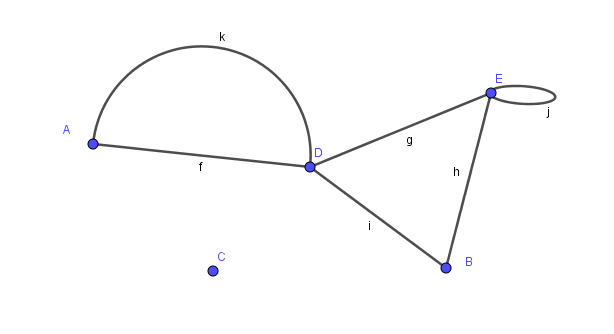
\includegraphics[width=0.55\linewidth]{8.png}
  \caption*{Fonte: Imagem Autoral.}
  \label{}
\end{figure}
\end{exemplo}

Utilizando esta definição, pode-se denominar outras características das estruturas de um grafo. Assim, por exemplo, estudamos: \textit{ordem, tamanho, incidência, adjacência, vizinhança, laço} e \textit{elo}. Assim, os separamos por tipos, como grafo: \textit{finito, nulo, simples, pseudografo, completo, conexo} e \textit{bipartido}. Dentre estas, observe as seguintes definições:

\begin{definicao}
Um grafo que não possui laços (arestas que possuem o mesmo vértice como extremidades),bem como não possui arestas paralelas (arestas cujas extremidades são os mesmo vértices) e onde quaisquer dois vértices são ligados por uma aresta é denominado \textit{grafo completo}.
\end{definicao}

\begin{definicao}
\textit{Grafo conexo} é o nome dado para o tipo de grafo onde é possível estabelecer um caminho de qualquer vértice para qualquer outro vértice dele. Caso contrário, temos um \textit{grafo desconexo}.
\end{definicao}

\begin{definicao}
Chamamos de \textit{grafo bipartido} o grafo onde pode-se particionar o conjunto de vértices em dois, de modo que cada aresta possua extremidades em ambos os conjuntos.
\end{definicao}

\begin{exemplo}
Exemplo de grafo bipartido:
\begin{figure}[h]
    \centering
    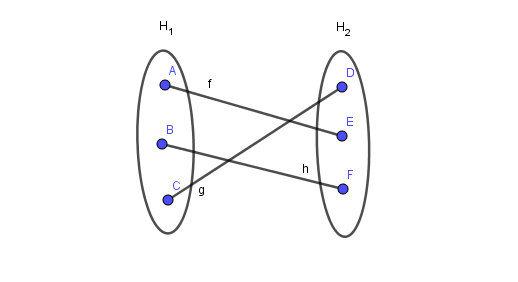
\includegraphics[scale=0.63]{10.png}
    \caption{Fonte: Imagem Autoral.}
    \label{figRotulo}
  \end{figure}
 \end{exemplo}
 
\begin{exemplo}
Exemplo de grafo conexo e completo:
\begin{figure}[h]
    \centering
    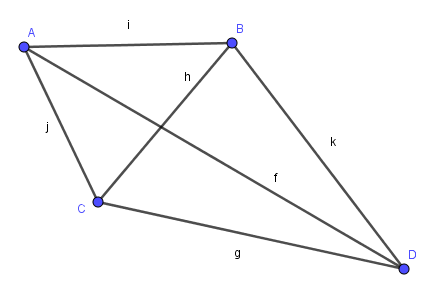
\includegraphics[scale=0.50]{Grafocompleto.png}
    \caption*{Fonte: Imagem Autoral.}
    \label{figRotulo}
  \end{figure}  
\end{exemplo}

Em diversos momentos o professor orientador buscou trazer perguntas acerca dos assuntos tratados. Neste caso, perguntas que surgiram foram:
\begin{enumerate}
\item Todo grafo conexo pode ser bipartido?
\item Todo grafo bipartido é conexo?
\end{enumerate}
A resposta é que nem todo grafo conexo pode ser bipartido, bem como nem todo grafo bipartido é conexo. Neste sentido, para verificar o primeiro item basta pegarmos qualquer grafo completo com 3 ou mais vértices e, uma vez que um dos conjuntos da bipartição terá mais de 2 vértices, com certeza teremos uma aresta cujas extremidades estarão num dos conjuntos da bipartição. Pelo Exemplo 2.1.2 podemos verificar que nem todo grafo bipartido é conexo, uma vez que partindo do vértice A, por exemplo, não podemos estabelecer um caminho até o vértice D.

Após este estudo, partiu-se para o estudo de \textit{subgrafos}. Em especial, foram discutidos \textit{caminhos} (tanto eulerianos quanto hamiltonianos), \textit{cliques, ciclos, árvores, dígrafos} e, por fim, \textit{grafos ponderados}. Aqui, é importante destacar a definição de \textit{grafo ponderado}, pois podemos representar os esquemas de distância atômica com base neles.

\begin{definicao}
Chamamos de \textit{grafo ponderado} o grafo que possui valores numéricos atribuídos as suas arestas.
\end{definicao}

Após isto, seguiu-se para o estudo de matrizes de incidência e adjacência. Assim, considere as seguintes definições:

\begin{definicao}
As extremidades de uma aresta são denominadas \textit{incidentes} à aresta, bem como esta aresta é \textit{incidente} às \textit{extremidades}.
\end{definicao}

\begin{definicao}
Vértices distintos e incidentes à uma mesma aresta são denominados \textit{adjacentes}. Nesse sentido, arestas que possuem um vértice em comum são \textit{adjacentes} também.
\end{definicao}

\begin{definicao}
Dois vértices distintos e adjacentes são denominados \textit{vizinhos}. O conjuntos de vértices \textit{vizinhos} geralmente é denotado por $N_{G}(v)$.
\end{definicao}

Assim, a partir de matrizes, é possível definir outras maneiras de representar um grafo.

\noindent\textbf{Matriz de Incidência: }Cada coluna representa os vértices incidentes a determinada aresta. Assim, cada linha representa as arestas incidentes a cada vértice. Contamos 1 para aresta incidente ao vértice (ou vice-versa) e 2 se tivermos um laço. Observe a matriz de incidência de $G_1$ à seguir:
\[
\begin{blockarray}{ccccccc}
f & g & h & i & j & k \\
\begin{block}{(cccccc)c}
  1 & 0 & 0 & 0 & 0 & 1 & A \\
  0 & 0 & 1 & 1 & 0 & 0 & B \\
  0 & 0 & 0 & 0 & 0 & 0 & C \\
  1 & 1 & 0 & 1 & 0 & 1 & D \\
  0 & 1 & 1 & 0 & 2 & 0 & E \\
\end{block}
\end{blockarray}
\]

\noindent\textbf{Matriz de Adjacência: }É uma tabela onde observa-se somente a relação de adjacência entre vértices. Caso um vértice seja adjacente a outro, bota-se número 1. No caso de um laço, bota-se 2. Observe a matriz de adjacência de $G_1$:
\[
\begin{blockarray}{cccccc}
A & B & C & D & E\\
\begin{block}{(ccccc)c}
  0 & 0 & 0 & 1 & 0 & A \\
  0 & 0 & 0 & 1 & 1 & B \\
  0 & 0 & 0 & 0 & 0 & C \\
  1 & 1 & 0 & 0 & 1 & D \\
  0 & 0 & 0 & 0 & 2 & E \\
\end{block}
\end{blockarray}
\]

Por último, foram estudados alguns resultados sobre \textit{grau de um vértice}. Assim, seguem outras definições, com a prova de 2 resultados na sequência.

\begin{definicao}
O \textit{grau} de um vértice é o número de arestas incidentes a ele. Cada laço conta como duas arestas. O vértice com \textit{grau} zero é chamado de \textit{vértice isolado}.
\end{definicao}
\begin{itemize}
\item $d_{G}(v)$: É o grau do vértice $v$. Se $G$ é um grafo simples (sem laços ou arestas paralelas), então $d_{G}(v)$ denota o número de vizinhos de $v$ em $G$.
\end{itemize}

\begin{teorema}
Para todo grafo $G(V(G),E(G))$, com $m$ arestas, vale:
$$
\sum\limits_{v\in V}{d_{G}(v)=2m}.
$$
\end{teorema}
\noindent\dem Considere a matriz de incidência M do grafo G. Para saber o grau de um determinado vértice basta olharmos para sua linha correspondente e somarmos os valores contidos na linha. Note que somar os valores presentes em todas as linhas é o mesmo que somar os valores presentes nas colunas. Como temos $m$ colunas e cada aresta possui 2 vértices incidentes, segue que $\sum\limits_{v\in V}{d_{G}(v)=2m}$.\qed

\begin{teorema}
Em qualquer grafo, o número de vértices, cujo grau é ímpar, é par.
\end{teorema}
\noindent\dem Suponha que o número de vértices com grau ímpar seja ímpar. Note que a soma do grau de todos os vértices resulta em um número ímpar(resultado aritmético). Somando este resultado com o grau dos demais vértices, cujo grau é par, obtemos um número ímpar. Absurdo, pois $\sum\limits_{v\in V}{d(v)=2m}$. Portanto, o número de vértices, cujo grau é ímpar, é par.\qed

\section{Problema de Geometria de Distâncias Moleculares (PGDM)}
Nesta etapa, encontros sem a presença do professor orientador foram recorrentes. O objetivo continuou sendo o mesmo, estudar os assuntos para apresentar os seminários. Entretanto, agora todos os alunos de iniciação científica estavam concentrados no estudo de \cite{1}. Além disso, quando necessário, o professor orientador pediu a implementação dos métodos sugeridos. Em diversos momentos surgiram dúvidas, comumente sanadas por revisões em \cite{algebralinear} e \cite{calculo}.

Inicialmente, foram vistos aspectos históricos sobre o PGDM. Seguindo, começou-se a trabalhar com os problemas. As hipóteses presentes em \cite{1} eram:

	\begin{itemize}
		\item Hipótese 1: as distâncias fornecidas pelos experimentos de RMN estão associados a pares de átomos conhecidos;
		\item Hipótese 2: todos os átomos da molécula da proteína cuja estrutura 3D queremos calcular são conhecidos;
		\item Hipótese 3: todos os átomos da molécula de proteína estão ligadas a algum átomo, cuja distância é conhecida;
		\item Hipótese 4: existe uma ordem, dada \textit{a priori}, entre os átomos da cadeia principal da proteína cuja estrutura 3D queremos calcular;
		\item Hipótese 5: as distâncias entre os átomos de uma molécula de proteína separados por duas ligações covalentes são conhecidas;
		\item Hipótese 6: as distâncias fornecidas pela RMN são representados por intervalos de números reais que contêm o valor correto associado.
	\end{itemize}

\noindent\textbf{Problema 2.2.1}: Encontrar os pontos $x_i\in\mathbb{R}^3$, com $i=1,\ldots,n$, que resolvam a seguinte equação:

$$||x_i -x_j||=d_{ij} , \forall\in E,
$$
onde $E \subset \{1, ...,n\} \times \{1, ...,n\}$ e os $d_{ij}$ são os valores de distâncias provenientes da Ressonância Magnética Nuclear (RMN).

Perceba que pode-se reescrever este problema em termos de otimização. Assim, segue que dado:

$$ f(x_1, ...,x_n) = \sum_{(i,j) \in E} (\|x_i - x_j\| - d_{ij})^2.
$$

Basta encontrar os $x_i \in \mathbb{R}^3$, $i = 1, ..., n$, tais que $f(x_1, ...,x_n)=0.$ Portanto, queremos
$$ \min_{x_t \in\mathbb{R}^n} f(x_1, ...,x_n).
$$

Na sequência, foi estudado um pouco sobre a geometria das proteínas. E, a partir das hipóteses 3 e 5, viu-se a possibilidade de utilizarmos coordenadas internas para resolver o problema, ao invés das cartesianas. Conforme a figura abaixo (presente na página 12 de \cite{1}), podemos representar uma proteína com base nos comprimentos das ligações covalentes $d_{i-1,i}$, ângulos planos $\theta_{i}$ e ângulos de torção $\omega_i$.

\begin{figure}[h]
    \centering
    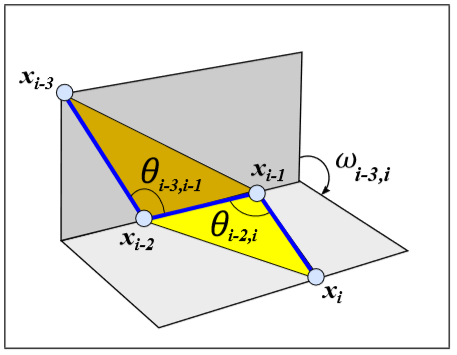
\includegraphics[scale=0.50]{angulos.png}
    \caption*{Fonte: ALVES. LAVOR. SOUZA. MACULAN. (2017). }
  \end{figure} 

Assim, considerando $x_i\in\mathbb{R}^3$, $i=1,\ldots,n$, dadas por $(x_{i1},x_{i2},x_{i3})$, podemos utilizar o seguinte método para determinar as coordenadas:

$$
\begin{bmatrix}
x_{i1}\\ 
x_{i2}\\ 
x_{i3}\\ 
1
\end{bmatrix}
= B_{1}B_{2}\cdots B_{i}\begin{bmatrix}
0\\ 
0\\ 
0\\ 
1
\end{bmatrix},
$$

onde

$$
B_1\: =\:
\begin{bmatrix}
1 & 0 & 0 & 0\\ 
0 & 1 & 0 & 0\\ 
0 & 0 & 1 & 0\\ 
0 & 0 & 0 & 1
\end{bmatrix},\:\:\:
\: B_2\: =\:
\begin{bmatrix}
-1 & 0 & 0 & -d_{1,2}\\
0 & 1 & 0 & 0\\ 
0 & 0 & -1 & 0\\ 
0 & 0 & 0 & 1
\end{bmatrix},
$$
$$
B_3\:=\:
\begin{bmatrix}
-\cos(\theta_{1,3}) & -\sin(\theta_{1,3}) & 0 & -d_{2,3}\cos(\theta_{1,3})\\ 
\sin(\theta_{1,3}) & -\cos(\theta_{1,3}) & 0 & d_{2,3}\sin(\theta_{1,3})\\ 
0 & 0 & 1 & 0\\ 
0 & 0 & 0 & 1
\end{bmatrix}
$$

e

$$
B_i\:=\:\scalemath{0.85}{
\begin{bmatrix}
-\cos(\theta_{i-2,i}) & -\sin(\theta_{i-2,i}) & 0 & -d_{i-1,i}\cos(\theta_{i-2,i})\\ 
\sin(\theta_{i-2,i})\cos(\omega_{i-3,i}) & -\cos(\theta_{i-2,i})\cos(\omega_{i-3,i})
 & -\sin(\omega_{i-3,i}) & d_{i-1,i}\sin(\theta_{i-2,i})\cos(\omega_{i-3,i})\\ 
\sin(\theta_{i-2,i})\sin(\omega_{i-3,i}) & -\cos(\theta_{i-2,i})\sin(\omega_{i-3,i}) & \cos(\omega_{i-3,i}) & d_{i-1,i}\sin(\theta_{i-2,i})\sin(\omega_{i-3,i})\\ 
0 & 0 & 0 & 1
\end{bmatrix},}
$$
com $i=4,\ldots,n$ para a última matriz.

Durante esta parte da iniciação científica, o aluno autor deste texto chegou num resultado interessante e que ajuda na compreensão geométrica de como o método funciona. Pode-se escrever a matriz $B_i$ do seguinte modo:

$$B_i=R_{x}(w_{i-3,i}).R_{x}(\pi).R_{z}(\theta_{i-2,i}).R_{y}(\pi).T_{x}(d_{i-1,i}),
$$
onde $R_{\alpha}(\gamma)$ representa a matriz de rotação que rotaciona um vetor por um ângulo $\gamma$ em torno do eixo $\alpha$, a partir da regra da mão direita. Além disso, $T_{\beta}(\lambda)$ representa uma translação de ``tamanho'' $\lambda$ em relação ao eixo $\beta$.  

Após isto, partiu-se para o estudo mais aprofundado sobre geometria de distâncias. Nesta parte, viu-se a relação entre grafos e o Problema de de Geometria de Distâncias Moleculares (PGDM), fato evidenciado pela seguinte definição (presente na página 21 de \cite{1}):

\begin{definicao}
Dado um grafo simples G=(V,E,d), conexo e ponderado nas arestas por $d:E\rightarrow(0,+\infty)$, encontre uma função $x:V\rightarrow\mathbb{R}^3$ tal que:

$$\forall\{u.v\}\in E, ||x(u)-x(v)||=d(u,v).$$
\end{definicao}
Assim, foi possível discutir o número de soluções PGDM e a complexidade computacional envolvida.

Por fim, este estudo deu a base necessária para a compreensão do algoritmo de Branch \& Prune, bem como permitiu que fossem feitas implementações computacionais. 
\chapter{Resultados e Discussão}
Em matemática é geralmente difícil para um aluno de graduação produzir conteúdo inédito. Assim, supõe-se que os maiores ganhos foram em experiência na atividade de pesquisa. 

O fato de existirem 5 membros na pequisa fez com que vários modos de pensar entrassem em conflito. Isto gerou um engrandecimento sobre a ideia de matemática que cada um tinha, além de permitir a produção de novos pontos de vista acerca dos principais tópicos.

\chapter{Considerações Finais}
Este projeto de iniciação científica exigiu muitos conhecimentos sobre Geometria Analítica e Álgebra Linear. Neste sentido, além de estar trabalhando com algo novo, foi uma oportunidade de consolidar o que já havia visto durante a graduação. Além disso, como o discente pretende seguir carreira acadêmica, foi um ótimo momento para estar em contato com o trabalho de um pesquisador.

Foi um período positivo em vários outros aspectos também. Amizades foram feitas e aprendeu-se a conversar sobre matemática. 

% ----------------------------------------------------------
% ELEMENTOS PÓS-TEXTUAIS
% ----------------------------------------------------------
% ----------------------------------------------------------
% ----------------------------------------------------------
% Referências bibliográficas
% ----------------------------------------------------------
    \postextual
    \bibliography{Refer_ncias.bib}
% ----------------------------------------------------------
% Glossário
% ----------------------------------------------------------
%
% Consulte o manual da classe abntex2 para orientações sobre o glossário.
%
%\glossary

% ----------------------------------------------------------
% Apêndices
% ----------------------------------------------------------

% ---
% Inicia os apêndices
% ---
% ---


% ----------------------------------------------------------
% Anexos
% ----------------------------------------------------------

% ---
% Inicia os anexos
% ---
%---------------------------------------------------------------------
% INDICE REMISSIVO
%---------------------------------------------------------------------
%\phantompart
\printindex
%---------------------------------------------------------------------

\end{document}
